\documentclass[14pt,a4paper]{report}  %紙張設定
\usepackage{xeCJK}%中文字體模組
\setCJKmainfont{標楷體} %中文字體
\newfontfamily\sectionef{Times New Roman}%設定英文字體
\usepackage{amsmath,amssymb}%數學公式、符號
\usepackage{graphicx, subfig}%圖形
\usepackage{graphicx, subfig}%圖片模組
\usepackage{type1cm} %調整字體絕對大小
\usepackage{textpos} %設定文字絕對位置
\usepackage[top=2.5truecm,bottom=2.5truecm,
left=2.5truecm,right=2.5truecm]{geometry}
\usepackage{titlesec} %目錄標題設定模組
\usepackage{titletoc} %目錄內容設定模組
\usepackage{CJK} %中文模組
\usepackage{CJKnumb} %中文數字模組
\usepackage{wallpaper} %浮水印
\usepackage{listings} %能加入程式碼
\usepackage{hyperref} %引用url連結
\usepackage{graphicx} %插入圖片
\usepackage{fontawesome5} %引用icon
%\linespread{1.5} %設定行距
\lstset{language=Python, %設定語言
		basicstyle=\footnotesize, 
		frame=lines,
		caption={Python code}, %設定capion
		label={lst:example} %設定label
}

\graphicspath{{./圖片/}} %圖片預設讀取路徑
\renewcommand{\figurename}{圖.} %設定圖片標示名稱
\renewcommand{\lstlistingname}{程式.} %設定程式標示名稱
 %=------------------更改標題內容----------------------=%
\titleformat{\chapter}[hang]{\sectionef\fontsize{20pt}{2.5pt}\bfseries}{\Large 第\CJKnumber{\thechapter}章}{1em}{}[]
\titleformat{\section}[hang]{\sectionef\fontsize{18pt}{2.5pt}\bfseries}{{\thesection}}{1em}{}[]
\titleformat{\subsection}[hang]{\sectionef\fontsize{18pt}{2.5pt}\bfseries}{{\thesubsection}}{1em}{}[]
%=------------------更改目錄內容-----------------------=%
\titlecontents{chapter}[0.25em]{}{\sectionef\fontsize{18pt}{2.5pt}\bfseries\makebox[3.5em][l]
{第\CJKnumber{\thecontentslabel}章}}{}{\titlerule*[0.7pc]{.}\contentspage}
\titlecontents{section}[18mm]{}{\sectionef\LARGE\makebox[1.5em][l]
{\thecontentslabel}}{}{\titlerule*[0.7pc]{.}\contentspage}
\titlecontents{subsection}[4em]{}{\sectionef\Large\makebox[2em][l]{{\thecontentslabel}}}{}{\titlerule*[0.7pc]{.}\contentspage}
%=----------------------標題-------------------------=%             
\begin{document} %文件
\begin{titlepage}%開頭
\begin{center}   %標題  
\makebox[1.5\width][s]
{\fontsize{24pt}{2.5pt}國立虎尾科技大學}\\[18pt]
\makebox[1.5\width][s]
{\fontsize{24pt}{2.5pt}機械設計工程系}\\[18pt]
\makebox[1.5\width][s]
{\fontsize{24pt}{2.5pt}專題製作報告}\\[18pt]
%設定文字盒子 [方框寬度的1.5倍寬][對其方式為文字平均分分布於方框中]\\距離下方18pt
\vspace{3em} %下移
\fontsize{30pt}{1pt}\textbf{強化學習在機電系統中之應用}\\

\vspace{4em}
\sectionef\fontsize{30pt}{1em}\textbf
{
\vspace{0.5em}
Application of reinforcement
 \vspace{0.5em} 
 learning in mechatronic systems}
 \vspace{2em}
%=---------------------參與人員-----------------------=%             
\end{center}
\begin{flushleft}
\begin{LARGE}
\hspace{32mm}\makebox[5cm][s]
{指導教授:\quad 嚴\quad 家\quad 銘\quad 老\quad 師}\\[6pt]
\hspace{32mm}\makebox[5cm][s]
{班\qquad 級:\quad 四\quad 設\quad 三\quad 甲}\\[6pt]
\hspace{32mm}\makebox[5cm][s]
{學\qquad 生:\quad 李\quad 正\quad 揚\quad(40723110)}
\\[6pt]
\hspace{32mm}\makebox[5cm][s]
{\hspace{36.5mm}林\quad 于\quad 哲\quad(40723115)}\\[6pt]
\hspace{32mm}\makebox[5cm][s]
{\hspace{36.5mm}黃\quad 奕\quad 慶\quad(40723138)}\\[6pt]
\hspace{32mm}\makebox[5cm][s]
{\hspace{36.5mm}鄭\quad 博\quad 鴻\quad(40723148)}\\[6pt]
\hspace{32mm}\makebox[5cm][s]
{\hspace{36.5mm}簡\quad 國\quad 龍\quad(40723150)}\\[6pt]
%設定文字盒子[寬度為5cm][對其方式為文字平均分分布於方框中]空白距離{36.5mm}\空白1em
\end{LARGE}
\end{flushleft}
\vspace{3em}
\fontsize{18pt}{2}\centerline{\makebox[\width][s]
{中華民國\hspace{3em} 
110 \quad 年\quad 3\quad 月}}
\end{titlepage}
\newpage
%=------------------------摘要-----------------------=%
\pagenumbering{roman}
\clearpage
\addcontentsline{toc}{chapter}{摘\quad 要} %將摘要加入目錄
\begin{center}
\LARGE\textbf{摘要}\\
\begin{flushleft}
\fontsize{14pt}{2.5pt}\hspace{12pt} 產業中需要加速許多工法的演算,以達到最佳化,但不能以實體一直測試不同方法,成本與時間不允許,便可以利用許多感測器觀測數值,以類神經網路運算,在虛擬環境架設結構,遠端控制、更改數值。\\
\vspace{1em}
\sectionef\fontsize{14pt}{2.5pt}\hspace{12pt} 此專題是利用現成裝置冰球台,設置對應虛擬模擬環境,減少現實模擬參數設置、成本,再加入類神經網路之中的 Policy gradient與Reinforcement Learning,訓練冰球達到對應最佳化。\\
\end{flushleft}
\begin{center}
\fontsize{14pt}{2.5pt}關鍵字:\sectionef Policy gradient、虛擬環境架設結構、Reinforcement Learning
\end{center}
\newpage
%=------------------------誌謝----------------------=%
\addcontentsline{toc}{chapter}{誌\quad 謝}
\centerline\LARGE\textbf{誌謝}\\
\begin{flushleft}
\fontsize{14pt}{2.5pt}\hspace{12pt}致謝內容
\end{flushleft}
\newpage
%=------------------------目錄----------------------=%
\renewcommand{\contentsname}{\centerline{\fontsize{18pt}{\baselineskip}\selectfont\textbf{目\quad 錄}}}
\tableofcontents  %目錄產生
\newpage
%=------------------圖表目錄產生----------------------=%
\renewcommand{\listfigurename}{\centerline{\fontsize{18pt}{\baselineskip}\selectfont\textbf{圖\quad 表\quad 目\quad 錄 }}}
\listoffigures
\newpage
\end{center}
%=-------------------------內容----------------------=%


\chapter{前言}
\pagenumbering{arabic} %設定頁號阿拉伯數字
\setcounter{page}{1}  %設定頁數
\fontsize{14pt}{2.5pt}\sectionef
\section{研究動機}
\qquad 機器學習與機電系統結合的運用越來廣泛,我們將其運用在桌球機上,使完成訓練的機電系統能獨自與玩家對打。\\
\section{研究目的與方法}
\qquad 本研究分兩大部分,第一運用Open AI Gym的Pong-v0來訓練機器學習,第二利用CoppilaSim模擬環境並訓練出能與人對打的機電系統。\\[12pt]
\qquad 利用Gym的訓練環境來側試不同的算法所得到的訓練結果,比較不同算法、參數間的差異,並找出較適合Pong game的算法、參數,循序漸進提高環境的真實程度,來減少一開始就是以實體的方式測試所帶來硬體、程式、時間和金錢等成本。\\[12pt]

\qquad 將Gym的訓練環境轉換到CoppilaSim模擬環境,利用貼近真實的模擬環境來修正在純程式的架構與真實環境間的誤差,雖然CoppilaSim模擬環境與真實環境仍有些微的落差,但與Gym相比CoppilaSim的環境已非常貼近真實了,拉近了虛擬與現實間的距離,提高了實用性的價值。\\

\section{未來展望}
\qquad 
\section{規則說明}
\qquad Pong game 的遊戲規則簡單,透過擊錘將球打入對方球門即得一分,只要其中一方得21分就結束該局。擊錘只能沿單方向來回移動來進行防守和進攻。\\[12pt]

遊戲規則如下:
\begin{enumerate}
\item 球打入敵方即得一分。
\item 擊錘只單一方向移動。
\item 最快贏得21分者獲勝,並結束該局遊戲。
\end{enumerate}

\chapter{機器學習的訓練方法}
\section{類神經網絡}
\qquad 類神經網路的概念來源是觀察人類的中樞神經系統而啟發的,類神經網路主要由多個節點組成,每個節點稱為神經元(neurons),神經元與神經元連結而形成的網路稱為神經網路。神經元主要又分成三層:輸入層(input layer)、隱藏層(hidden layer)和輸出層(output layer)。神經元會接收上一層的訊號,並經過啟動函數(activation function)計算並輸出至下一層神經元。神經網路輸入層的神經元負責接收訊號,透過隱藏層來運算,再傳遞到輸出層執行動作。由於每個神經元經過啟動函數的非線性計算,所以神經元傳出的數值也是非線性。神經元與神經元間連線在生物學稱為突觸(Synapse),在數學模型裡每個突觸都有權重(weights)。在既定框架下,調配權重值和啟動函數會使結果更接近預期。神經網路的架構指標為以下幾項:階層數、每層神經元個數、神經元連接方式、啟動函數的類型等。\\[12pt]

\qquad 神經訊號傳遞分為前饋(feed-forward)和回饋(backpropagation)。前饋為傳遞經過啟動函數計算的數值。回饋則是修正權重和偏差(biases),以提高下次前饋計算的準確度。
\subsection{啟動函數}
以下介紹幾種較為常見的啟動函數及其特性:
\begin{itemize}
%=----------Sigmoid      Function----------=%
\item Sigmoid Function:\\
輸出介於0到1之間,適用於二元分類,方程式具有非線性、可連續微分、並具有固定輸出範圍等特性,並可以讓類神經網路呈現非線性。\\
$$\sigma(x)=\frac{1}{1+e^{-x}}$$ \\[6pt]
\iffalse
\begin{figure}[hbt!]
\begin{center}
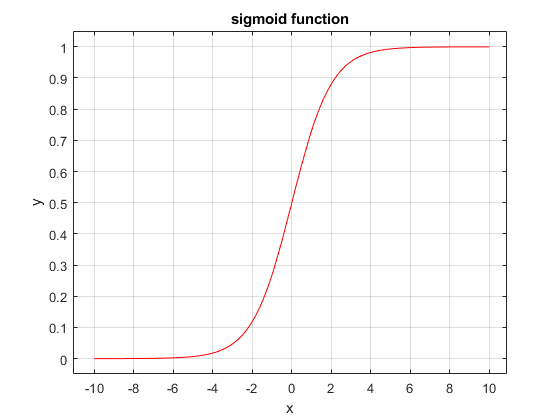
\includegraphics[scale=0.74]{sigmoid_function}
\caption{Sigmoid; 
from: \href{https://towardsdatascience.com/derivative-of-the-sigmoid-function-536880cf918e}{Toward Data Science}}
\end{center}
\end{figure}
\fi
%=----------SigmoidPrime Function----------=%
SigmoidPrime Function是從Sigmoid Function微分得來,以梯度運算的方式,可以減少梯度誤差,但也是造成梯度消失的主要原因,若要改善梯度消失需要搭配優化器使用,方程式如下:\\[12pt]
$$\sigma^{'}(x)=\sigma(x)[1-\sigma(x)]$$\\[3pt]
%=----------Softmax Function----------=%
\item Softmax:\\
Softmax會計算每個事件分布的機率,適用多項目分類、其機率總合為1。以此專案為例,假設擊錘移動有向上移動、向下移動及不移動這三個決策選項,則這三個決策機率值總和為1。\\[12pt]
$$S(x)=\frac{e^{x_i}}{\sum^k_{j=1}e^{x_i}}$$
%=----------Relu Function----------=%
\item ReLU Function:\\
ReLU Function方程式特性:若輸入值為負值,輸出值為0;若輸入值為正值,輸出則維持該輸入數值。ReLU計算方式簡單、收斂速度快,這是類神經網路最普遍拿來使用的啟動函數,因為可以解決梯度消散的問題,但須注意:起始值若設定到不易被激活範圍或是權重過度所導致權重梯度為0就會造成神經元難以被激活。
$$f(x)=max(0,x)$$
$$if , x<0 , f(x)=0$$
$$else f(x)=x$$\\
%=----------Adam Function----------=%
\item Adam Function\\
結合了 Adagrad 和 RMSprop的優勢,有論文表示,在訓練速度方面有巨大性的提升,但在某些情況下,Adam實際上會找到比隨機梯度下降法更差的解決方法。以下是計算過程: \\[6pt]
$$g_t=\delta_{\theta}f(\theta)$$\\
一次矩指數移動均線 :\\[6pt]
 $$m_t =\beta(m_{t-1})+(1-\beta_1)(\nabla{w_t})$$\\
$$\hat m_t=\frac{m_t}{1-\beta_1^t}$$\\[6pt]
二次矩指數移動均線 :\\[6pt]
$$v_t=\beta_2(v_t-1)+(1-\beta_2)(\nabla{w_t})^2$$\\
$$\hat{v_t}=\frac{v_t}{1-\beta_2^t}$$\\
因此,Adam Function:\\[6pt]
\begin{Large}$$\omega_{t-1}=\omega_t-\frac{\eta}{\sqrt{\hat{v_t}-\epsilon}}\hat{m_t}$$\end{Large}
%=----------Mean Squared Error----------=%
\item Mean Squared Error\\
他能告訴你一組點與回歸線接近的程度,透過獲取點與回歸線之距離(這些距離就是誤差)並對它們進行平方來做到這點,而平方是為了消除所有負號,也能讓更大的差異賦予更大的權重。
(\href{https://www.statisticshowto.com/mean-squared-error/}{\underline{Extracted from here)}}.\\[6pt]
\begin{figure}
\center
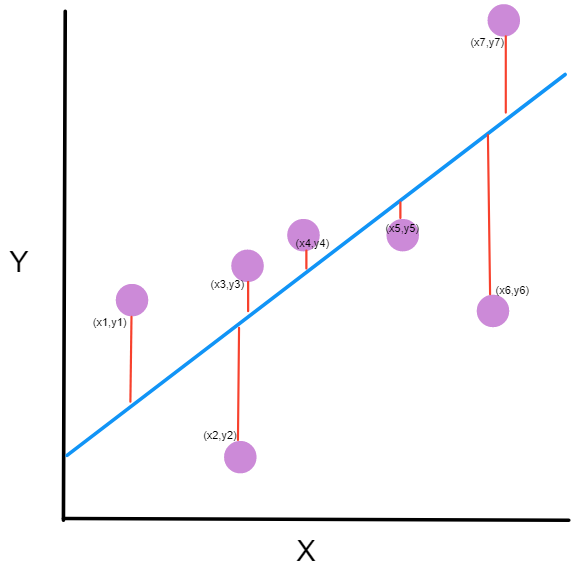
\includegraphics[height=7cm]{MSE}
\caption{regression line}
\end{figure}

回歸線 :數據點間最小距離的一條線。 \\
n : 數據點的數量\\
$y_i$ :  觀測值\\
$\hat{y_i}$ : 預測值\\
\begin{Large}
$$MSE=\frac{1}{n} \sum_{i=1}^n(y_i-\overline{y} _i)^2$$
\end{Large}\\[6pt]
\end{itemize}

\iffalse %整段註解(開頭)
% 以下為 SigmoidPrime的證明
%$$-------------skip-------------$$
Tip: find $f^{'}(x)$ if $f(x)=\frac{A}{B+Ce^{x}}$\\
Answer:\\
$$\frac{d}{dx}[\frac{1}{g(x)}]=\frac{1^{'}g(x)-1g^{'}(x)}{g(x)^2}=\frac{g^{'}(x)}{[g(x)]^2}$$\\
if $g(x)$=constant\\
$$\frac{d}{dx}[\frac{g(x)}{h(x)}]=\frac{g^{'}(x)h(x)-g(x)h^{'}(x)}{h(x)^2}= \frac{-kh^{'}(x)}{[h(x)]^2}$$\\
$$f^{'}(x)=\frac{-A[\frac{d}{dx}(B+Ce^x)]}{(B+Ce^x)^2}=\frac{-A(0+Ce^x)}{(B+Ce^x)^2}=\frac{-ACe^x}{(B+Ce^x)^2}$$\\[6pt]
$$-------------skip-------------$$\\[6pt]
Hence:\\
$$=-(1+e^{-x})^{-2}\frac{d}{dx}(1+e^{-x})=-(1+e^{-x})^{-2}[\frac{d}{dx}(1)+\frac{d}{dx}(e^{-x})]$$\\
$$=-(1+e^{-x})^{-2}[0+\frac{d}{dx}(e^{-x})]=-(1+e^{-x})^{-2}[\frac{d}{dx}(e^{-x})]=-(1+e^{-x})^{-2}[e^{-x}\frac{d}{dx}(-x)]$$\\
$$-(1+e^{-x})^{-2}[e^{-x}(-1)]=-(1+e^{-x})^{-2}(-e^{-x})=\frac{e^{-x}}{(1+e^{-x})^2}=\frac{1(e^{-x})}{(1+e^{-x})(1+e^{-x})}$$\\
$$=\frac{1}{1+e^{-x}}\frac{e^{-x}}{1+e^{-x}}=\frac{1}{1+e^{-x}}\frac{e^{-x}+1-1}{1+e^{-x}}=\frac{1}{1+e^{-x}}(\frac{1+e^{-x}}{1+e^{-x}}-\frac{1}{1+e^{-x}})$$\\[6pt]


\begin{figure}[hbt!]
\begin{center}
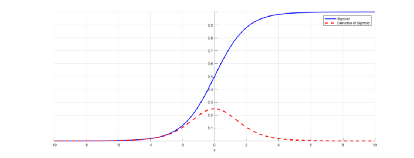
\includegraphics[scale=0.80]{sigmoidprime}
\caption{SigmoidPrime; from: \href{https://towardsdatascience.com/derivative-of-the-sigmoid-function-536880cf918e}{Toward Data Science}}
\end{center}
\end{figure}


%\begin{figure}[hbt!]
%\begin{center}
%\includegraphics[height=4.5cm]{relu}\\
%\caption{Relu; from : \href{https://www.kaggle.com/dansbecker/rectified-linear-units-relu-in-deep-learning}{\underline{kaggle}} }
%\end{center} 
%\end{figure}

\newpage
\end{itemize}
\fi %整段註解(結尾)
\subsection{優化器}
\qquad 為了讓機器學習的錯誤率降低,因此利用優化器來降低loss function的值,在error surface上找到最小值,即是找到錯誤率最低的地方。也可以改善啟動函數梯度消失的問題,以下將介紹幾種優化的方法:
\begin{itemize}
\item Gradient Descent\\[6pt]
利用梯度的方式尋找最小值的位置,其特色可找到凸面error surface的絕對最小值,在非凸面error surface上找到相對最小值。其缺點是在非凸面error surface要避免被困在次優的局部最小值。\\
\item Batch gradient descent\\[6pt]
用批次的方式計算訓練資料,整個資料集計算梯度只更新一次,因此計算和更新時會占用大量記憶體。整體效率較差、速度較緩慢。由 Gradient Descent 延伸出來的算法。其收斂行為與 Gradient Descent 相同。\\
\item Stochastic gradient descent\\[6pt]
每次執行時會更新並消除誤差,有頻繁更新和變化大的特性,較不容易困在特定區域。由 Gradient Descent 延伸出來的算法。其收斂行為與 Gradient Descent 相同。\\
\item Mini-batch gradient descent\\[6pt]
結合 Batch gradient descent 和 Stochastic gradient descent 的特點:批量計算和頻繁更新,所衍伸的算法。利用小批量的方式頻繁更新,並使收斂更穩定。其缺點:學習率挑選不易、預定義 threshold 無法適應數據集的特徵、對很少發生的特徵無法執行較大的更新、非凸面error surface要避免被困在次優的局部最小值等。\\
\item Gradient descent optimization algorithms\\[6pt]
為了改善前面幾種算法而發展出來的優化算法。以下將列出數種優化算法。\\
\item Momentum\\[6pt]
在梯度下降法加上動量的概念,會加速收斂到最小值並減少震盪。\\
\item Nesterov accelerated gradient\\[6pt]
NAG,有感知能力的 Momentum:在坡度變陡時減速,避免衝過最小值所造成的震盪(為了修正到最小值,來回修正而產生的震盪)\\
\item Adagrad\\[6pt]
其學習率能適應參數:頻繁出現的特徵用較低的學習率,不經常出現的特徵則用較高的學習率,且無須手動調整學習率。其缺點是,學習率會急遽下降,最後會無限小,這算法就不再獲得知識。\\
\item Adadelta\\[6pt]
為 Adagrad 的延伸,下降激進程度,學習率從更新規則中淘汰,不需設定預設學習率。\\
\item RMSprop\\[6pt]
為了解決 Adagrad 學習率急劇下降的問題,學習率除以梯度平方的RMS,解決學習率無限小的情形。\\
\item Adam\\[6pt]
類似 Momentum,更加穩定快速的收斂。\\
\item AdaMax\\[6pt]
與 Adam 相似,依靠$(u_t)$ 最大運算。\\
\item Nadam\\[6pt]
結合 Adam 和 NAG ,應用先前參數執行兩次更新,一次更新參數一次更新梯度。\\
\item AMSGrad\\[6pt]
改善 Adam 算法所導致收斂較差的情況(用指數平均會減少其影響),換用梯度平方最大值來做計算,並移除去偏差的步驟。是否有比 Adam 算法好仍有待觀察。\\
\item Gradient noise\\[6pt]
有助於訓練特別深且復雜的網絡,noise 可改善不良初始化的網路。\\
\end{itemize}
\section{深度學習}
%=----------deep learning 會在此時崛起?----------------=%

\qquad 深度學習的崛起與電腦科學有著密切的關係,四個主要趨勢為:\\
\begin{enumerate}
\item 支援張量運算程式語言與程式庫的崛起\\[6pt]
首先,自從1960年代開始,諸如APL、MATLAB、R和Julia等領域的特定語言的發展轉變為多為數組(通常稱為張量) 進入一組由全為數學語(或運算符)支援的第一類物件以對其進行操作此外,基於數組的編程能夠以通用語言(如 Python、Lisp、C++和Lua)高校運作,諸如NumPy、Torch、Eigen和Lush等。\\

\item 自動求導數套件的開發\\[6pt]
其次,自動微分的發展使得完全自動化計算導數的艱鉅工作成為了可能, 這使的運用不同的機器學習方法進行實驗變得非常容易,同時仍然允許基於梯度的優化。 因為autograd軟件包的普及,並將該技術用於NumPy數組,並且類似的方法也用於框架中,例如: Chainer, DyNet, Lush, Torch, Jax and Flux.jl。\\

\item 自由開源軟體的普及\\[6pt]
第三隨著自由軟件的到來,科學界從封閉的專用軟件(例如Matlab)轉向開源, Python的生態系統,帶有NumPy、SciPy和Pandas等軟件包,滿足了大多數研究人員對數值分析需求,同時讓他們能夠利用龐大的程式庫來處理數據集的預處理,例如:統計分析、繪圖等。\\
此外,自由軟體的開放性、互相操作性和靈活性,促進了充滿活力的社會發展,這樣社會可以通過擴展程式庫現有的功能,或著在需要時通過開發和發布全新的程式庫功能,來迅速滿足新的或不斷變化的需求。 儘管有豐富的非Python語言支持的神經網路開源軟件,從Lish中的Lush、C++中的Torch、Objective-C和Lua、C++中的EBLearn、C++中的Caffe開始,大型生態系統(諸如Python)的網路效應,促使研究快速發展成為一項必不可少的技能。因此,自2014年以來,大多數深度學習的框架都將Python介面作為一項基本功能進行融合。\\

\item 多核 GPU 運算的發展 \\[6pt]
最後,利用大規模通用硬體(例如GPU)的可能性,提供深度學習方法所需的計算能力、專用的程式庫(例如:cuDNN)以及大量學術著作(例如Andrew Lavin、maxdnn:使用maxwell gpus進行深度學習的高效卷積內核、2015年1月以及Andrew Lavin和Scott Gray用於卷積神經網路的快速算法、2016年IEEE電腦視覺和圖形識別(CVPR),第4013-4021頁,2016), 產生了一系列高性能可重用的深度學習內核,這些內核使諸如Caffe,Torch7, or TensorFlow 的框架能夠利用這些硬體加速器。\\
\end{enumerate}

\newpage
\section{強化學習}
%=----------What is Reinforcement Learning?------------=%
強化學習是通過agent(代理)與已知或未知的環境持續互動,不斷適應與學習,得到的回饋可能是正面,也就是獎賞(reward),如果得到負面,那就是懲罰(punishments)。考慮到agent與環境(environment)互動,進而決定要執行哪個動作,強化學習的學習模式是建立在獎賞與懲罰上。\\[6pt]
%====================須修改====================%
強化學習與其他學習法不一樣的地方在於:不需要事先收集大量數據提供當作學習樣本,而是透過與環境互動,在環境下發生的狀態當作學習的來源。
與其他機器學習不同,因為我們不需要在意訓練數據集。互動不是發生在數據上,而是在環境下發生,通過互動描繪出真實的場景。由於強化學習是建立在環境的,因此許多參數進行運算,需要大量信息來學習,並根據此採取行動。強化學習的環境是真實世界,可能是2D或3D模擬世界的場景,也可能是建立於遊戲的場景。從某種意義上來說,強化學習的範圍很廣,因為環境的規模可能很大,並且在環境中有多相關因素,影響著彼此。強化學習的目的是達到目標。強化學習的獎勵是來自環境。
%=----------Faces of Reinforcement Learning---------------=%
\begin{itemize}
\item 強化學習涵蓋範圍\\

%======需文字補充========%
\begin{figure}[hbt!]
\begin{center}
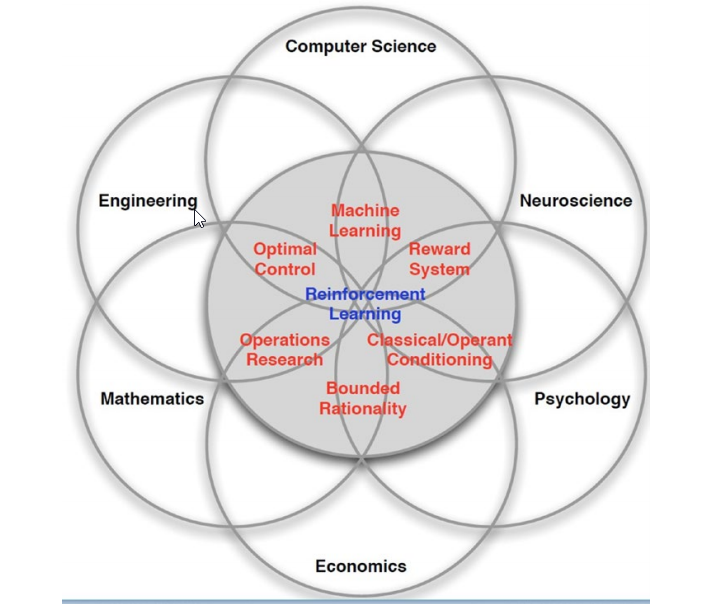
\includegraphics[scale=0.74]{Faces_of_Reinforcement_Learning}
\caption{Venn diagram; }%from: \href{file:///H:/201906_fall/data/tmp/project2020-1/downloads/reinforcement_learning/2018_Book_ReinforcementLearning.pdf}{All the faces of Reinforcement Learning}
\end{center}
\end{figure}
%=--------The Flow of Reinforcement Learning------------=%.

\item  強化學習的流程\\

\begin{figure}[hbt!]
\begin{center}
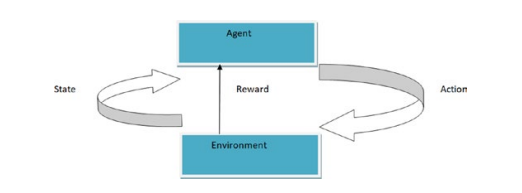
\includegraphics[width=10cm]{The_Flow_of_Reinforcement_Learning}
\caption{RL structur}
\end{center}
\end{figure}
\textbf{需要考慮的重點:}
\item 強化學習的週期是互相聯繫的
\item 分明的溝通是在考慮獎勵的情況下發生的
\item agent與環境之間存在著獨特的溝通。
\item 目標或機器人從一狀態移動到另一狀態。
\item 從一狀態轉移到另一種狀態採取動作。

\begin{figure}[hbt!]
\begin{center}
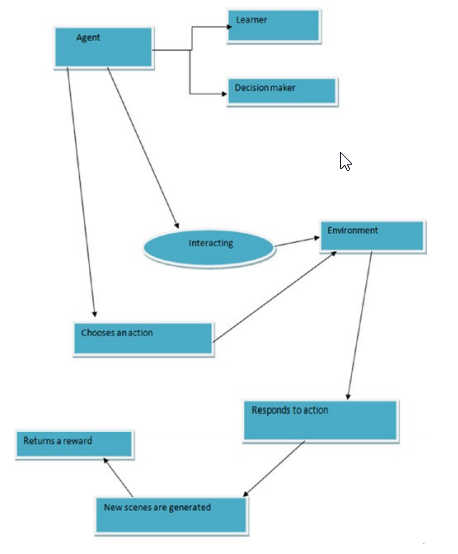
\includegraphics[width=15cm]{The_entire_interaction_process}
\caption{The entire interaction process; }%from: \href{file:///H:/201906_fall/data/tmp/project2020-1/downloads/reinforcement_learning/2018_Book_ReinforcementLearning.pdf}{All the faces of Reinforcement Learning}
\end{center}
\end{figure}
agent是決策者,因為他會試圖採取獲得最高大獎勵的行動。\\
當agent開始與環境互動時,他可以選擇一個操作並做出相應的回應,從這時起,將會創建新的場景,當agent從一個環境變為另一個環境中,每項更改都會導致某種修改,這些變化被描述為場景,每個步驟中發生的過度都有助於agent更有效地解決強化學習的問題。\\

%------------------圖片可共用----------------------%
%\begin{figure}[hbt!]
%\begin{center}
%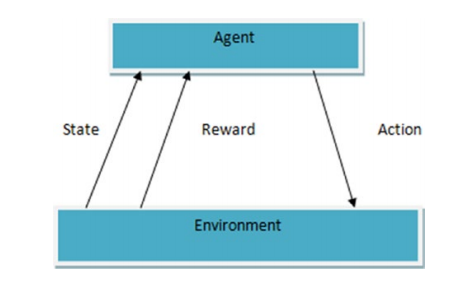
\includegraphics[scale=0.74]{Scenario_of_state_changes}
%\caption{The entire interaction process; }%from: \href{file:///H:/201906_fall/data/tmp/project2020-1/downloads/reinforcement_learning/2018_Book_ReinforcementLearning.pdf}{All the faces of Reinforcement Learning}
%\end{center}
%\end{figure}

%=----Different Terms in Reinforcement Learning----------=%

\item 強化學習中各種術語\\
在此情況下,有兩個很重要的常數-$\gamma$、$\lambda$\\[10pt]
$\gamma$用於每個狀態轉換,且在每次狀態變化時,都是一個恆定值, 
$\gamma$ 會從你將在每個狀態獲得的獎勵類型中,告訴你訊息。$\gamma$又叫衰減因子,他決定了我們未來可獲得的獎勵類型:\\
\item  $\gamma$值為0表示獎勵僅與當前狀態有關係。
\item$\gamma$值為1時,代表獎勵是長期的。
當我們處理時間問題時,通常使用$\lambda$,這是涉及更多的連續狀態的預測,
每種狀態下的$\lambda$值增加,代表我們的算法學習速度很快,適用強化學習技術時,更快的算法會產生更好的結果。\\
%=----Interactions with Reinforcement Learning------------=%
\item 與強化學習的互動\\
%------------------圖片可共用----------------------%
%\begin{figure}[hbt!]
%\begin{center}
%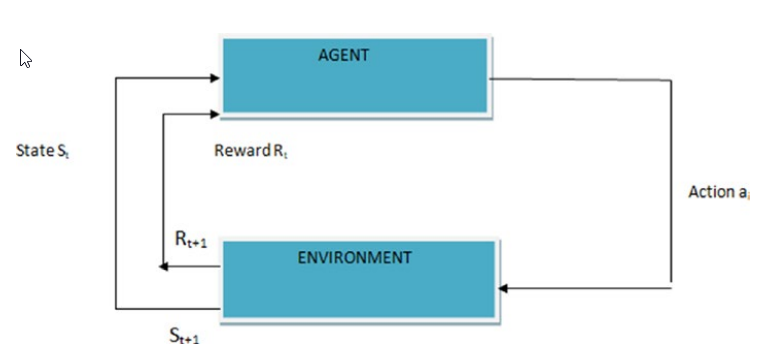
\includegraphics[scale=0.74]{ Reinforcement_Learning_interactions}
%\caption{Reinforcement Learning interactions; }%from: \href{file:///H:/201906_fall/data/tmp/project2020-1/downloads/reinforcement_learning/2018_Book_ReinforcementLearning.pdf}{All the faces of Reinforcement Learning}
%\end{center}
%\end{figure}

agent和環境之間的互動會產生獎勵,我們採取行動,從一種狀態轉移到另一種狀態\\
強化學習是一種實現如何將情況映設為行動的方法,從而最大化並找到獲得最高獎勵的方法
,機器或機器人不會像其他機器學習形式的機器人那樣被告知要採取哪些行動,但機器必須發現哪些動作會產生最大的獎勵。\\
%=----How Reward Works------------=%

\item 獎勵如何運作\\

獎勵是我們從一狀態過渡到另一狀態時所獲得的動力,它可以是分數,例如在遊戲中。我們訓練的次數越多,我們就變得越精準,且我們的回報越大。\\
%=----Agents------------=%
\item Agents\\
在強化學習方面,agent是一個軟體程式,能做出明智的選擇,應能購感知到正在環境發生的事情,以下是agent基本步驟:\\
\item 當agent可以感知環境時,它可以做出比以往更好的決定。
\item agent採取的決定就會產生行動。
\item agent執行的行動必須是最好最佳的。
\begin{figure}[hbt!]
\begin{center}
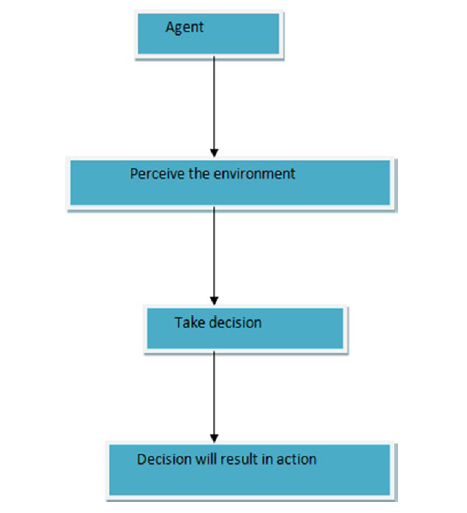
\includegraphics[scale=0.74]{agent}
\caption{agent}%from: \href{file:///H:/201906_fall/data/tmp/project2020-1/downloads/reinforcement_learning/2018_Book_ReinforcementLearning.pdf}{All the faces of Reinforcement Learning}
\end{center}
\end{figure}
%=----Agents------------=%
\item 強化學習的環境\\
強化學習中的環境由某些因素組成,會對agent產生影響,agent必須根據環境適應其各種因素,並做出最佳決策,這些環境可以是2D世界或是網格,甚至是3D世界。\\
\begin{large}textbf{以下是環境的一些重要功能:}\end{large}\\
\item 具有確定性。
\item 可觀察性。
\item 是離散或是連續的狀態。
\item 單個agent或是多個agent。
\end{itemize}

\newpage
\section{深度強化學習}
\subsection{Deep Reinforcement Learning}
\begin{figure}[hbt!]
\begin{center}
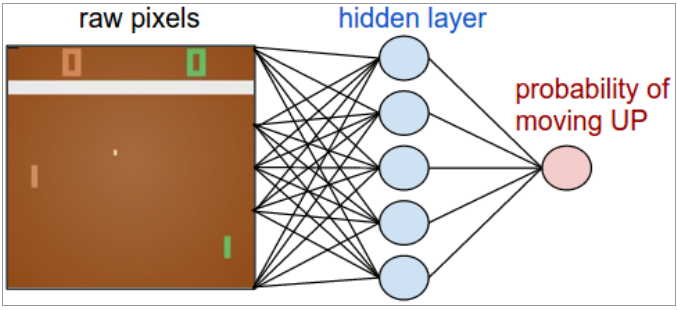
\includegraphics[scale=0.74]{ network}
\caption{Our network is a 2-layer fully-connected net. }%from: \href{file:///H:/201906_fall/data/tmp/project2020-1/downloads/reinforcement_learning/2018_Book_ReinforcementLearning.pdf}{All the faces of Reinforcement Learning}
\end{center}
\end{figure}\textbf{}

\qquad 我們將定義一個可以執行我們的玩家(agent)的類神經網路,該網路將獲取遊戲狀態並決定我們應該做什麼(向上移動或向下移動
) 我們使用一個2層神經網路,該網路獲取原始圖像像素(100,800個數字(210*160*3)),並生成一個表示上升概率的數字。 使用隨機策略是標準做法,這意味著我們只會產生向上移動的可能性,每次迭代時,我們都會從該分布中採樣(即扔一枚有偏見的硬幣)已獲得實際移動。\\


\subsection{Supervised Learning}
\begin{figure}[hbt!]
\begin{center}
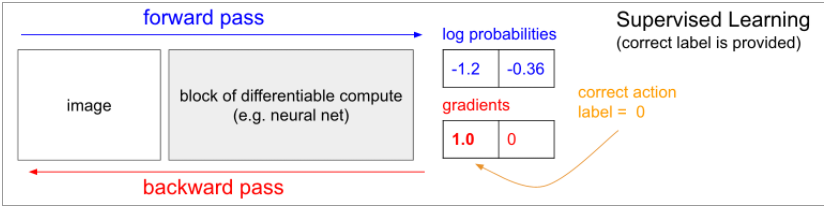
\includegraphics[scale=0.74]{supervising_learning}
\caption{supervising learning }%from: \href{file:///H:/201906_fall/data/tmp/project2020-1/downloads/reinforcement_learning/2018_Book_ReinforcementLearning.pdf}{All the faces of Reinforcement Learning}
\end{center}
\end{figure}\textbf{}

\qquad 在我們滲入探討 Score Function 解決方案之前,需要簡短介紹有關監督學習的知識,因為正如我們看到的,與我們架構類似,在普通通的監督學習中,我們會將圖像送到網路,並獲得伊些概率,例如對於兩個類別的上和下。 這裡顯示的是向上和向下對數概率(-1.2,-0.36),而不是原始機率(在這個情況下,是30$\%$和70$\%$),因為我們總是優化正確標籤的對數概率(這使我們的演算法更好,病等效於優化原始概率,因為對數是單調的),而在監督學習中,我們將可以獲取標籤,例如:\\

我們可能被告知現在正確的做法是向上運動(標籤0),在執行過程中,我們將以上的對數機率輸入1.0的梯度,然後運行backprop來計算梯度向量$Wlogp(y=UP|x)$這個梯度將告訴我們應如何更改百萬個參數中的每個參數,使網路預測往上的可能性更高,例如:網路中的百萬個參數之一可能具有-2.1的梯度,這意味著如果我們將該參數增加一個小的正值(例如0.001),則往上的對數機率將因2.1*0.001而降低(由於負號而減少),如果我們隨後更新了參數,當之後遇到非常相似的圖像時(也就是環境狀況),我們的網路現在更有可能預測往上。\\

\subsection{對數導數技巧}
\qquad 機器學習涉及操縱機率。這個機率通常包含normalised-probabilities或 log-probabilities。能加強解決現代機器學習問題的關鍵點,是能夠巧妙的在這兩種型式間交替使用,而對數導數技巧就能夠幫助我們做到這點,也就是運用對數導數的性質。\\
\subsection{Score Functions}
\qquad 對數導數技巧的應用規則是基於參數$\theta$梯度的對數函數$p(x:\theta)$,如下:\\
$$\nabla_\theta logp(x:\theta)=\frac{\nabla_\theta p(x:\theta)}{p(x:\theta)}$$\\
$p(x:\theta)$是likelihood ; function參數$\theta$的函數,它提供隨機變量x的概率。在此特例中,$\nabla_\theta logp(x:\theta)$被稱為Score Function,而上述方程式右邊為score ratio(得分比)。\\[6pt]

\begin{large}
{score function具有許多有用的屬性:}
\end{large}
\begin{itemize}
\item 最大概似估計的中央計算。最大概似是機器學習中使用的學習原理之一,用於廣義線性回歸、深度學習、kernel machines、降維和張量分解等,而score出現在這些所有問題中。
\end{itemize}
\begin{itemize}
\item  score的期望值為零。對數導數技巧的第一個用途就是證明這一點。\\
$$\mathbb{E}_{p(x; \theta)}[\nabla_\theta \log p(\mathbf{x}; \theta)] =\mathbb{E}_{p(x; \theta)}\left[\frac{\nabla_\theta p(\mathbf {x}; \theta)}{p(\mathbf{x}; \theta)} \right]$$
$$= \int p(\mathbf {x}; \theta) \frac{\nabla_\theta p(\mathbf {x}; \theta)}{p(\mathbf{x}; \theta)} dx= \nabla_\theta \int p(\mathbf{x}; \theta) dx=\nabla_\theta 1 = 0$$\\
\qquad 在第一行中,我們應用了對數導數技巧,在第二行中,我們交換了差異化和積分的順序,這種特性是我們尋求概率靈活性的類型:  它允許我們從期望值為零的分數中減去任何一項,且此修改不會影響預期得分(控制變量)。
\end{itemize}
\begin{itemize}
\item 得分的方差是Fisher信息,用於確定Cramer-Rao下限。\\
$$\mathbb{V}[\nabla_\theta \log p(\mathbf{x}; \theta)] = \mathcal{I}(\theta) =\mathbb{E}_{p(x; \theta)}[\nabla_\theta \log p(\mathbf{x}; \theta)\nabla_\theta \log p(\mathbf{x}; \theta)^\top]$$\\
我們現在可以從對數概率的梯度躍升為概率的梯度,然後返回,但是真正要解決的其實是計算困難的期望梯度,所以我們可以利用新發現的功能:score function為此問題開發另一個聰明的估計器。
\end{itemize}
\subsection{Score Function Estimators}
我們的問題是計算函數f的期望值的梯度:\\
$$\nabla_\theta \mathbb{E}_{p(z;\theta)}[f(z)] =\nabla_\theta \int p(z; \theta)f(z) dz$$\\

這是機器學習中的一項常態性任務,在變數推理中進行後驗計算,在強化學習中進行價值函數和策略學習,在計算金融中進行衍生產品定價以及在運籌學中進行庫存控制等。該梯度很難計算,因為積分通常是未知的,我們計算梯度所依據的參數θ的分佈為p(z;θ),此外,當函數f不可微時,我們可能想計算該梯度,使用對數導數技巧和得分函數的屬性,我們可以更方便地計算此梯度:\\
$$\nabla_\theta \mathbb{E}_{p(z;\theta)}[f(z)] = \mathbb{E}_{p(z;\theta)}[f(z)\nabla_\theta \log p(z;\theta)]$$\\

\begin{figure}[hbt!]
\begin{center}
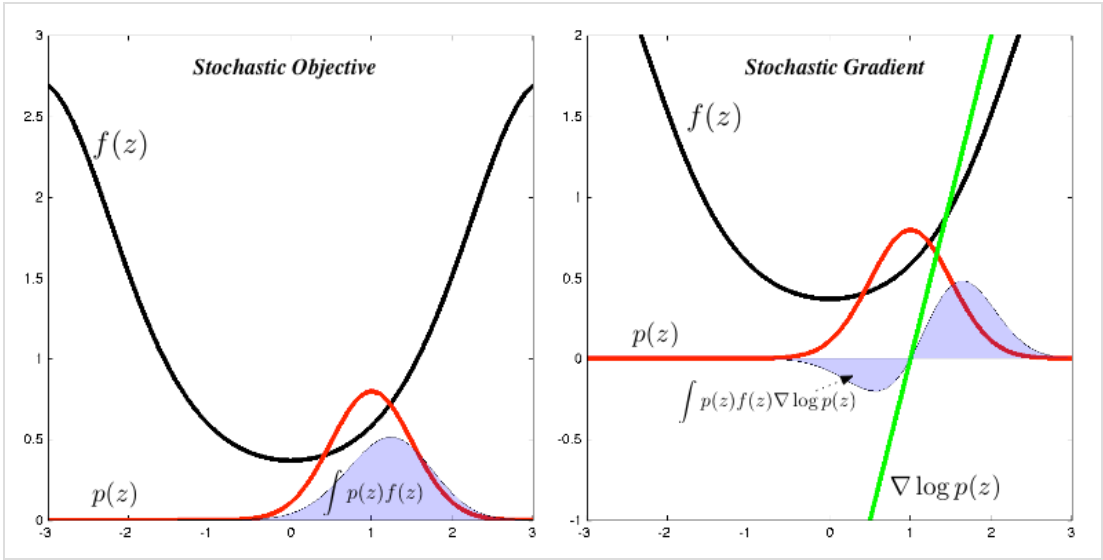
\includegraphics[scale=0.5]{gradient_change}
\caption{gradient change}%from: \href{file:///H:/201906_fall/data/tmp/project2020-1/downloads/reinforcement_learning/2018_Book_ReinforcementLearning.pdf}{All the faces of Reinforcement Learning}
\end{center}
\end{figure}
\qquad 讓我們導出該表達式,並探討它對我們的優化問題的影響。\\
\qquad 為此,我們將使用另一種普遍存在的技巧,一種概率恆等的技巧,在該技巧中,我們將表達式乘以1,該表達式由概率密度除以自身而形成。將特性技巧與對數導數技巧相結合,我們獲得了梯度的得分函數估計量:\\
$$\nabla_\theta \mathbb{E}_{p(z;\theta)}[f(z)]=\int\nabla_\theta p(z;\theta)f(z) dz$$\\[6pt]
$$= \int \frac{p(z;\theta)}{p(z;\theta)}\nabla_\theta p(z;\theta)f(z) dz$$\\[6pt]
$$=\int p(z;\theta)\nabla_\theta \log p(z;\theta)f(z) dz = \mathbb{E}_{p(z;\theta)}[f(z)\nabla_\theta \log p(z;\theta)]$$\\[6pt]
$$=\int p(z;\theta)\nabla_\theta \log p(z;\theta)f(z) dz = \mathbb{E}_{p(z;\theta)}[f(z)\nabla_\theta \log p(z;\theta)]$$\\[6pt]
$$\approx \frac{1}{S} \sum_{s=1}^{S}f(z^{(s)})\nabla_\theta \log p(z^{(s)};\theta) \quad z^{(s)}\sim p(z)$$\\[6pt]
在這四行中發生了很多事情。在第一行中,我們交換了導數和積分。在第二行中,我們應用了概率身份技巧,這使我們能夠形成得分比, 然後使用對數導數技巧,用第三行中對數概率的梯度替換該比率。這在第四行給出了我們所需的隨機估計量,這是由蒙特卡洛計算的,方法是首先從p(z)提取樣本,然後計算加權梯度項。.\\

更簡單的描述,我們有一些分佈 $p(x;\theta)$(我使用了速記$ p(x)$來減少混亂),我們可以從中採樣(例如,這可能是高斯)。對於每個樣本,我們還可以評估分數函數f,該函數將樣本作為樣本並給出標量值。該方程式告訴我們,如果我們希望其樣本達到較高的分數(由f判斷),應該如何改變分佈(通過其參數θ),特別是,它看起來像:畫出一些樣本x,評估其分數f(x),並且對於每個x也評估第二項 $\nabla_\theta logp(x;θ)$,那第二項是什麼,它是一個向量-漸變為我們提供了參數空間中的方向,這將導致分配給x的概率增加。換句話說,如果我們要在的方向上微移θ,$\nabla_\theta logp(x;θ)$,我們會看到分配給x的新概率略有增加。如果回顧一下公式,它告訴我們應該朝這個方向發展,並將標量值加到上面$f(x)$。這樣一來,得分較高的樣本將比那些得分較低的樣本“拖拉”更強的概率密度,因此,如果我們要根據p上的幾個樣本進行更新,則概率密度將朝著較高分數的方向移動,從而使得分較高的樣本更有可能出現。\\
\begin{figure}[hbt!]
\begin{center}
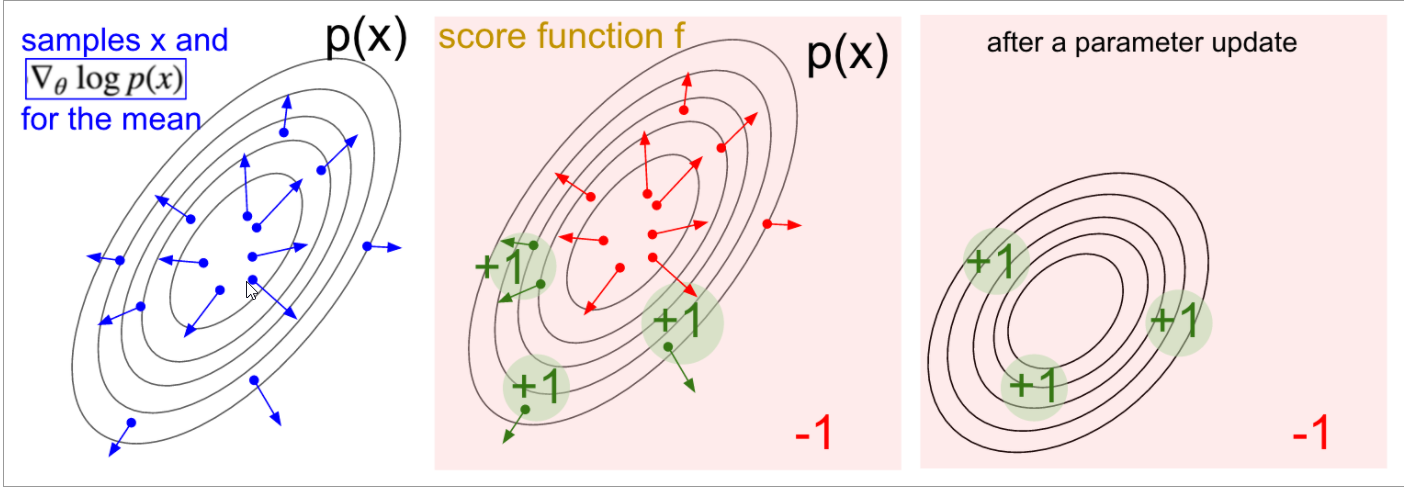
\includegraphics[scale=0.4]{figure}
%\caption{gradient change}%from: \href{file:///H:/201906_fall/data/tmp/project2020-1/downloads/reinforcement_learning/2018_Book_ReinforcementLearning.pdf}{All the faces of Reinforcement Learning}
\end{center}
\end{figure}
\qquad score function gradient estimator的可視化,左:高斯分佈及其中的一些樣本(藍點),在每個藍點上,我們還繪製了相對於高斯平均參數的對數概率的梯度,箭頭指示應微調分佈平均值以增加該樣本概率的方向。中間:某些得分函數的疊加,在某些小區域中除了+1之外,其他所有地方都給出-1(請注意,這可以是任意的,不一定是可微分的標量值函數),箭頭現在採用了顏色區別,因為由於更新中的乘法運算,我們將平均所有綠色箭頭和紅色箭頭的負數。右:更新參數後,綠色箭頭和反向紅色箭頭將我們向左移至底部。現在,根據需要,該分佈中的樣本將具有更高的預期分數。\\
\newpage
\section{比較個方法的特色}
\newpage
\chapter{馬可夫決策}

\section{Markov Chain}
\quad 當前決策只會影響下個狀態,當前狀態轉移(action)到其他狀態的機率有所差異。
\section{Markov Reward Process}
\quad action 到指定狀態會獲得獎勵。
$$R(s_t=s) = \mathbb{E}[r_t|s_t = s]$$
$$\gamma \in [0, 1]$$
\begin{itemize}
\item Horizon:\\
在無限的狀態以有限的狀態表示\\
\item Return:\\
越早做出正確決策獎勵越高\\
$$G_t = R_{t+1}+\gamma R_{t+2}+\gamma^2 R_{t+3}+\gamma^3 R_{t+4}+...+\gamma^{T-t-1} R_{T}$$

\item State value function:\\
決策價值\\
$$V_t(S) = \mathbb{E}[G_t|s_t = s]$$
\begin{center}
\hspace{-4em}\makebox[\width][s]{$P(s_{s+1}=s'|s_t=s,a_t=a)$}
\end{center}
\end{itemize}

\section{Markov Decision Process}
\quad 在MRP中加入決策(decision)和動作(action)\\
\begin{itemize}
\item S:state 狀態
\item A:action 動作
\item P:狀態轉換\\[6pt]
\begin{center}
\hspace{-4em}\makebox[\width][s]{$P(s_{s+1}=s'|s_t=s,a_t=a)$}
\end{center}

\end{itemize}
\newpage
\chapter{訓練環境}
\section{openAI Gym}
\qquad Gym 是用於開發和比較強化學習算法的工具包,他不對agent的結構做任何假設,並且與任何數據計算庫兼容,而可以用來制定強化學習的算法。這個環境具有共享的介面,使我們能用來編寫常規算法,也就能教導agents如何步行到玩遊戲。\\[6pt]


\section{Pong}
\qquad 取自 1977年發行的一款家用遊戲機ATARI 2600中的遊戲,內建於Gym,這是一個橫向的乒乓遊戲,左方是遊玩者,右邊是馬可夫決策的特例,每個邊緣都會給予reward(figue1),目標就是計算再任意階段動作最佳路徑,已獲得rewardd最大值。
\section{為什麼選擇score function 算法}
\qquad 多篇論文已經廣泛使用了ATARI遊戲並結合了DQN(它是一種在強化學習算法裡,知名度較高的),事實證明,Q-Learning並不是一個很好的算法,實際上大多數人比較喜歡使用Policy Gradients,包括原始DQN論文的作者,他們在調優後顯示Policy Gradients比Q 首選PG,因為它是端到端的:有一個明確的政策和一種有原則的方法可以直接優化預期的回報。但是礙於時間考量,而選擇了類似PG的算法,也就是score function gradient estimator(取用Andrej Karpathy),從像素開始,通過深度神經網絡使用ATARI遊戲(Pong),並在整個過程結合numpy,作為訓練工具。


\section{Pong from pixels}
\qquad 左:乒乓球遊戲。右:Pong是Markov決策過程(MDP)的特例:圖,其中每個節點都是特定的遊戲狀態,每個邊緣都是可能的(通常是概率性的)改變,每條邊界都給與獎勵,目標是計算在任何狀態下發揮作用的最佳方式,以最大限度地提高獎勵。\\ 
Pong的遊戲是簡單的強化學習中,很好的例子,在ATARI 2600版本中,我們會控制右邊邊的操縱板(左邊由不錯的AI控制)。在較低級別上,遊戲的運行方式如下:我們收到一個圖像幀(一個210x160x3 byte數組(從0到255的整數給出像素值)),然後決定是否要向上或向下移動操縱板(即二進制選擇)。每次選擇之後,遊戲模擬器就會執行動作並給予我們獎勵:如果球超過了對手,則為+1獎勵;如果我們錯過球,則為-1獎勵;否則為0。當然,我們的目標是移動球拍,以便獲得很多獎勵。\\

\newpage
\chapter{模擬環境}
\section{模擬模型}
\qquad 在模擬的模型上,延用了學長設計的冰球機,並進行了部分的設計變更,將原本的人機對打更改為機器對打,且因為搭配神經網路的訓練,所以將兩邊的擊球器都僅保留X軸向(左右)移動,而冰球則是使用原本設計。多虧了學長們所設計的冰球機模型,讓我們在運作上有問題時可以直接發問,設計變更的地方也可以快速完成。\\
\section{CoppeliaSim模擬}
\qquad CoppeliaSim是具有集成開發環境的機器人模擬器,基於分佈式控制體系架構,可以通過嵌入式腳本,插件,ROS或BlueZero節點,RemoteAPI客戶端或自定義解決方案進行模型控制。\\
\subsection{使用原因}
\qquad 本專題之最終目標是希望可以將訓練完成的AI可以在虛擬環境中進行模擬測試,通過虛擬環境中的模擬後,可以更直接地看到神經網路訓練的狀況,且因為在虛擬環境中不會有金費的支出,所以可以不斷的重複模擬直到模擬達到最佳的狀態,基於以上原因,所以使用了CoppeliaSim協助開發。\\
\subsection{模擬}
\begin{enumerate}

\item 功能說明\\

 以下為簡易功能說明:\\
 
\item 模擬執行\\

\end{enumerate}
\subsection{CoppeliaSim中的Vision sensor}

\section{影像處理}
\qquad 在影像處理中我們主要使用了Python套件中的OpenCV(全稱:Open Source Computer Vision Library),並搭配其他套件或模組進行了影像處裡,藉此來取得訓練神經網路訓練時所需的資訊。\\
\subsection{影像辨識}
\qquad 透過CoppeliaSim中的Vision sensor接收場景影像並輸出後,便可以開始進行影像辨識的處裡\\
\begin{enumerate}
\item RGB與HSV的轉換\\

RGB即光的三原色Red(紅)Green(綠)Blue(藍),HSV則是一種將RGB色彩模型中的點在圓柱坐標系中的表示法,HSV分別表示Hue(色相)、Saturation(飽和度)、Value(明度)\\



\item 顏色過濾\\

進行顏色過濾時,需要先定義出過濾顏色的上下限,在開始過濾後低於下限或高於上限的值會變成0(即黑色),而介於上下限範圍間的值會變成255(即白色)\\

\item 雜訊去除\\

為了避免環境因素干擾,使影像產生雜訊並影響了影像辨識度,所以在雜訊的去除也是很重要的,
\end{enumerate}
\newpage
\chapter{伺服器}
\begin{itemize}
\item Oracle VM VirtualBox\\
\qquad 因應在虛實整合需要用到虛擬環境去模擬的情況,我們使用 Ubuntu 當作我們的作業系統去建構虛擬環境,而在此之前要先安裝「虛擬機器工作站」— Oracle VM VirtualBox 。
\section{Oracle VM VirtualBox 介紹}
當要使用不同的的作業系統 ( Linux , Ubuntu , Red Hat ...  ) 而不想與其資料存放時共用一個硬碟 ( 沒有多餘硬碟 , 不想硬碟之間有資料重疊 ... ) 時,就可以使用其軟體做練習,降低操作失誤帶來的成本,而此軟體目前為免費,並隨時會更新,另外其特色有 :
\item 只要自備作業系統 ( 光碟片 , ISO映像檔 ) ,即可在啟動 Oracle VM VirtualBox  後直接開啟要操作的執行檔 ( 作業系統 ),不必再把主機本身重新關機,當然開啟多個作業系統之間也有共通性,可直接從視窗A做網路、檔案分享、複製貼上等動作到視窗B。
\item 除了作業系統裡面的執行,還可在其中練習磁碟分割、格式化以及 BIOS 啟動等 ( 但是未支援USB啟動 ) 。
\item 空間的佔用上並不是真實佔用空間,而是依據使用者的操作而變化 ( 使用者用多少就是多少 )。相對的,使用者雖然一開始設定該虛擬電腦的記憶體大小與硬碟空間是實時依據操作者決定,但終究還是佔掉電腦效能,所以 VirtualBox 的效能還是依據電腦本身的硬體配備
\item
\end{itemize}
\newpage
\chapter{深度強化學習的訓練與控制}
程式訓練流程:\\

\qquad 擷取影像,將影像裁剪至實際遊戲範圍,並簡化像素以利提高訓練時的計算速度,減少運算時的負擔,過濾顏色只保留球與擊錘,並把取到的影像二元化,取兩幀畫面進行比較,掌握球與擊錘間的相對位置(畫面差),透過前饋:計算球在環境的狀態及擊錘移動的決策,畫面差透過W1權重來計算球在環境的狀態,透過W2權重並經過啟動函數(activation function)得出擊錘移動的決策。透過產生隨機值的方式來與擊錘移動決策值進行比較,隨機值若落在決策向上移動的區間,擊錘就會向上移動;落在決策向下移動的區間,就會進行該動作。計算discount reward及獎勵的加總。\\

\qquad 在單局結束時,紀錄下該局累積下來的經驗,亦是紀錄該局所修正出來的參數而進行獎勵計算、log probability、\\
\newpage
\chapter{問題與討論}
Q:啟用cmsimde的MathJax的功能遇到文章使用括號補充說明的內容被誤當成latex的語法轉換。\\

A:格式轉換原始定義成"("和")",所以出現誤換的問題。\\
\begin{lstlisting}
<script>
  MathJax = {
    tex: {inlineMath: [['$', '$'], ['\\(', '\\)']]}
  };
  </script>
  <script id="MathJax-script" async src="https://cdn.jsdelivr.net/npm/mathjax@3/es5/tex-chtml.js"></script>
\end{lstlisting}
修正後將"("和")"換成"\$",就解決誤換問題
%=---------------------參考文獻----------------------=%
\newpage
\begin{center}
\addcontentsline{toc}{chapter}{參考文獻 }
\LARGE\textbf 參考文獻\\
\end{center}
\begin{flushleft}
\begin{Large}
[1]\quad https://towardsdatascience.com/derivative-of-the-sigmoid-function-536880cf918e\\

[2]\quad https://towardsdatascience.com/adam-latest-trends-in-deep-learning-optimization-6be9a291375c\\
\end{Large}
\end{flushleft}
\newpage
\begin{center}
\LARGE\textbf 作者簡介\\
\end{center}

\framebox[8cm][r]{\vspace{1em}test}


\end{document}